\documentclass{article}

\usepackage[english]{babel}
\usepackage[letterpaper,top=2cm,bottom=2cm,left=3cm,right=3cm,marginparwidth=1.75cm]{geometry}
\usepackage{amsmath}
\usepackage{graphicx}

% Definir caminho das imagens
\graphicspath{{Arquivos/imagens/}}

\title{Your Paper}
\author{You}

\begin{document}
\maketitle

\begin{abstract}
Your abstract.
\end{abstract}

\section{Introduction}

Your introduction goes here! Simply start writing your document and use the Recompile button to view the updated PDF preview.

\section{Some examples to get started}

\subsection{How to include Figures}

First you have to upload the image file from your computer. Then use the includegraphics command to include it in your document. See the code for Figure \ref{fig:frog} below.

\begin{figure}[h]
  \centering
  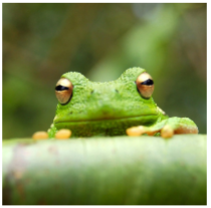
\includegraphics[width=0.6\textwidth]{frog.png}
  \caption{This frog was uploaded via the file-tree menu.}
  \label{fig:frog}
\end{figure}

As you can see in Figure \ref{fig:frog}, the image is now included in the document.

\subsection{How to add Tables}

Use the table and tabular environments for basic tables --- see Table~\ref{tab:widgets}, for example.

\begin{table}[h]
\centering
\begin{tabular}{l|r}
Item & Quantity \\\hline
Widgets & 42 \\
Gadgets & 13
\end{tabular}
\caption{An example table.}
\label{tab:widgets}
\end{table}

\subsection{How to add Lists}

You can make lists with automatic numbering:

\begin{enumerate}
\item Like this,
\item and like this.
\end{enumerate}

Or bullet points:
\begin{itemize}
\item Like this,
\item and like this.
\end{itemize}

\subsection{How to write Mathematics}

\LaTeX{} is great at typesetting mathematics. Let $X_1, X_2, \ldots, X_n$ be a sequence of independent and identically distributed random variables with $\text{E}[X_i] = \mu$ and $\text{Var}[X_i] = \sigma^2 < \infty$, and let
\[S_n = \frac{X_1 + X_2 + \cdots + X_n}{n}
      = \frac{1}{n}\sum_{i}^{n} X_i\]
denote their mean.

\section{Conclusion}

We hope you find this document useful!

\end{document}

